%%%%%%%%%%%%%%%%%%%%%%%%%%%%
%                          %
% Luther Michaels          % 
% ECE 351-52               %
% Lab 3                    %
% September 23, 2021       %
% Discrete Convolution     %
%           Lab Report     %
%                          %
%%%%%%%%%%%%%%%%%%%%%%%%%%%%

%%%%%%%%%%%%%%%%%%%%%%%%%%%%%%%%%%%%%%%%%%%
%%% DOCUMENT PREAMBLE %%%
\documentclass[12pt]{report}
\usepackage[english]{babel}
\usepackage{url}
\usepackage[utf8x]{inputenc}
\usepackage{amsmath}
\usepackage{graphicx}
\graphicspath{{images/}}
\usepackage{parskip}
\usepackage{fancyhdr}
\usepackage{vmargin}
\usepackage{listings}
\usepackage{hyperref}
\usepackage{xcolor}

\definecolor{codegreen}{rgb}{0,0.6,0}
\definecolor{codegray}{rgb}{0.5,0.5,0.5}
\definecolor{codeblue}{rgb}{0,0,0.95}
\definecolor{backcolour}{rgb}{0.95,0.95,0.92}

\lstdefinestyle{mystyle}{
	backgroundcolor=\color{backcolour},   
	commentstyle=\color{codegreen},
	keywordstyle=\color{codeblue},
	numberstyle=\tiny\color{codegray},
	stringstyle=\color{codegreen},
	basicstyle=\ttfamily\footnotesize,
	breakatwhitespace=false,         
	breaklines=true,                 
	captionpos=b,                    
	keepspaces=true,                 
	numbers=left,                    
	numbersep=5pt,                  
	showspaces=false,                
	showstringspaces=false,
	showtabs=false,                  
	tabsize=2
}

\lstset{style=mystyle}

\setmarginsrb{3 cm}{2.5 cm}{3 cm}{2.5 cm}{1 cm}{1.5 cm}{1 cm}{1.5 cm}

\title{3}	% Title						
\author{Luther Michaels}	% Author		
\date{September 23, 2021}   % Date

\makeatletter
\let\thetitle\@title
\let\theauthor\@author
\let\thedate\@date
\makeatother

\pagestyle{fancy}
\fancyhf{}
\rhead{\theauthor}
\lhead{\thetitle}
\cfoot{\thepage}
%%%%%%%%%%%%%%%%%%%%%%%%%%%%%%%%%%%%%%%%%%%%

\begin{document}
	
%%%%%%%%%%%%%%%%%%%%%%%%%%%%%%%%%%%%%%%%%%%%%%%%%%%%%%%%%%%%%%%%%%%%%%%%%%%%%%%%%%
%%% TITLE PAGE %%%
\begin{titlepage}
	\centering
	\vspace*{0.5 cm}
	
	\begin{center}    
		\textsc{\Large   ECE 351 - Section \#52}\\[2.0 cm]	
	\end{center}  
	\textsc{\Large Discrete Convolution  }\\[0.5 cm]
	\rule{\linewidth}{0.2 mm} \\[0.4 cm]
	{ \huge \bfseries \thetitle}\\
	\rule{\linewidth}{0.2 mm} \\[1.5 cm]
	\begin{minipage}{0.4\textwidth}
		\begin{flushleft} \large
		\end{flushleft}
		\end{minipage}~
	\begin{minipage}{0.4\textwidth}
		\begin{flushright} \large
			\emph{Submitted By:} \\
			Luther Michaels \break
			
			\emph{Submission Date:} \\
			September 23, 2021
		\end{flushright}
	\end{minipage}\\[2 cm]
\end{titlepage}
	
%%%%%%%%%%%%%%%%%%%%%%%%%%%%%%%%%%%%%%%%%%%%%%%%%%%%%%%%%%%%%%%%%%%%%%%%%%%%%%%%%%
%%% TABLE OF CONTENTS %%%
	
\tableofcontents
\pagebreak
	
%%%%%%%%%%%%%%%%%%%%%%%%%%%%%%%%%%%%%%%%%%%%%%%%%%%%%%%%%%%%%%%%%%%%%%%%%%%%%%%%%%
%%% LAB REPORT %%%
\renewcommand{\thesection}{\arabic{section}}
\section{Introduction}
	
The central concept to be examined in this lab is convolution. The goal is to implement and test a user-defined convolution function in Python in order to better understand the fundamentals and characteristics of the operation. This procedure utilizes the user-defined step and ramp functions created in the previous lab experiment. The function scipy.signal.convolve will be used to verify the user-defined convolution. Two useful tools throughout this process are numpy.exp which applies an exponential function, and numpy.append that allows values to be added to the end of a numpy array. All functions and plots can be produced using Python code written within the Spyder software with the necessary imported packages.
	
\section{Equations}
	
\begin{equation}
	u(t)=
	\begin{cases}
		0 & t < 0\\
		1 & t\ge 0\\
	\end{cases}
\end{equation}
\begin{equation}
	r(t)=
	\begin{cases}
		0 & t < 0\\
		t & t\ge 0\\
	\end{cases}
\end{equation}
\begin{equation}
	f_1(t)= u(t - 2) - u(t - 9)
\end{equation}
\begin{equation}
	f_2(t)= e^{-t} u(t)
\end{equation}
\begin{equation}
	f_3(t)= r(t - 2)[u(t - 2) - u(t - 3)] + r(4 - t)[u(t - 3) - u(t - 4)]
\end{equation}
\begin{equation}
	y(t)= h(t) * x(t) = \int_{0}^{t}h(\tau)x(t - \tau)d\tau
\end{equation}

\section{Methodology}
	
The first step of the procedure, detailed in Part 1 of the lab outline, requested three user-defined functions be created using step and ramp functions as well as an exponential. The three functions were written by first copying the user-defined step and ramp from the prior lab; these were used in the definition alongside numpy.exp from the numpy Python package for the exponential. The three functions implemented Equations 3, 4, and 5. The code below shows both these three functions and the constant step size for good resolution referenced in each portion of the experiment. The functions' time intervals were established between 0 and 20 seconds using numpy.arange. A single plot with subplots for each function, a title, and axis labels was created with matplotlib.pyplot package commands. \\
	
\begin{lstlisting}[language=Python]
""" Part 1, Task 1: USER-DEFINED FUNCTIONS"""
def f_1(t):   # time input
	f = u(t - 2) - u(t - 9) # Function built from step function u(t).
	return f   # function return

def f_2(t):   # Exponential implemented with numpy package.
	f = np.exp(-t) * u(t) 
	return f  

def f_3(t):    # Function built using u(t) and ramp function r(t).
	f = (r(t - 2) * (u(t - 2) - u(t - 3))) + (r(4 - t) * (u(t - 3) - u(t - 4)))
	return f 

steps = 1e-2    # step size
t = np.arange(0, 20 + steps, steps)   # time interval: [0,20]
\end{lstlisting}
	
In Part 2 of the lab outline, the task was to write a user-defined convolution function in Python. The solution offered here was presented by the lab TA. The method began by capturing the lengths of the input functions as variables. These functions and their lengths were used to create two arrays using numpy.append that housed the input functions. The process of copying each function into another array's lowest indicies and padding any length disparity with zeros was necessary to ensure that both function arrays were of equal size. This size would be the combination of the original function lengths and was uniform out of necessity for the two to be analyzed together at each point. The function continued by creating a final array to store the result; its size could be made equal to the dimension size of either extended array. \\ 

By this step, both inputs and the output were set up to cover the same time interval. The procedure to take the convolution followed its mathematical expression shown in Equation 6. Given that integration is a sum of the area under a function, the setup in this equation was altered to replace the integral with a summation. An outer loop iterated through the combined size of the function lengths, while an inner was created to pass through only the original input function size. \\

Reflecting back on Equation 6, the index of this outer loop acted as the time t and the inner as $\tau$. Whenever the two overlapped such that the length of both functions combined (t) was greater than that of the single function ($\tau$), the multiplication of the two functions evaluated at $\tau$ and t - $\tau$ was added to the growing sum at that value of time. The sums at each index totaled the overlap to form the convolution integral. The time interval for the convolution result could not utilize the original time declaration since the function returned an array of the combined function size. Consequently, a second time was initialized to match the return dimensions that spanned nearly twice the original time interval. \\

\begin{lstlisting}[language=Python]
""" Part 2, Task 1: USER-DEFINED CONVOLUTION  """
def conv(f1, f2):
	Nf1 = len(f1) # Length of input functions stored in variables.
	Nf2 = len(f2)
	
	# Two arrays of equal length created from input functions.
	f1Extended = np.append(f1, np.zeros((1, Nf2 - 1)))  
	# -1 since index starts at 0
	f2Extended = np.append(f2, np.zeros((1, Nf1 - 1)))  
	# Buffer array with zeros for a size combining both functions.
	result = np.zeros(f1Extended.shape) 
	# Create a result array of same size using reference f1.
	   
	# Iterate through combined size.
	for i in range(Nf2 + Nf1 - 2): # -2 since each index starts at 0
	  # Iterate through original function size of f1.
		for j in range(Nf1): # same function as when creating result
			# condition: length of both functions is greater than first
			if((i - j + 1) > 0):   # +1 as index starts at 0
				try:
			  	# Result sum increased by product of evaluated functions.
					result[i] += f1Extended[j] * f2Extended[i - j + 1]
			  			# accumulation of area of overlap
				except:       
					print(i,j)  # error checking
	return result

t_2 = np.arange(0, (40 + (2 * steps)), steps) # expanded interval
\end{lstlisting}

The final lab requirement was to verify the functionality of the user-defined convolution function. In addition to the numpy and matplotlib.pyplot Python packages, scipy.signal was necessary to accomplish this task. Using the same plotting procedure, the three possible convolutions of the user-defined functions were graphed using both the new function and scipy.signal.convolve. \\

Github Link: \url{https://github.com/Luther-Michaels}
	
\section{Results}

The three user-defined functions were plotted together in a single figure shown below. Each is provided over the time interval between 0 and 20s. The first function is clearly an accurate model of the corresponding equation as it steps up at 2s and back down at 9s. The second, likewise, is a standard exponential decay as expected. The third function is a ramp up at 2s and back down to 4s that matches the mathematical prescription. The plots show that the time step is small enough to achieve sufficient resolution. \\
	
\begin{center}
	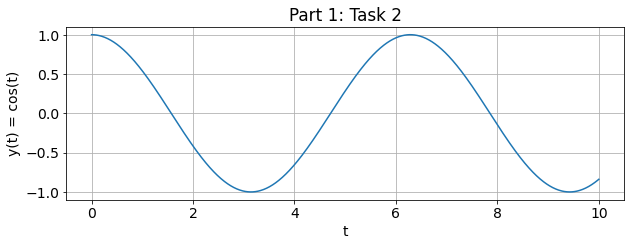
\includegraphics[scale = 0.6]{Part1-Task2.png}\\[1.0 cm]
\end{center}

The following three plots show the possible convolution combinations of these functions. The first convolves $f_1(t)$ with $f_2(t)$. If we consider a graphical convolution of the two, we might flip the exponential around the y-axis and shift it right with time. This would produce overlap that gradually grows before sharply decreasing as the functions pass. Not only does the result match our intuition, it also matches the Python package convolution function shown in the bottom subplot. It is also evident that the time interval has been extended since the structure of the user-defined convolution function combines the two input lengths. Thus, the original upper bound of 20s is now 40s. \\

\begin{center}
	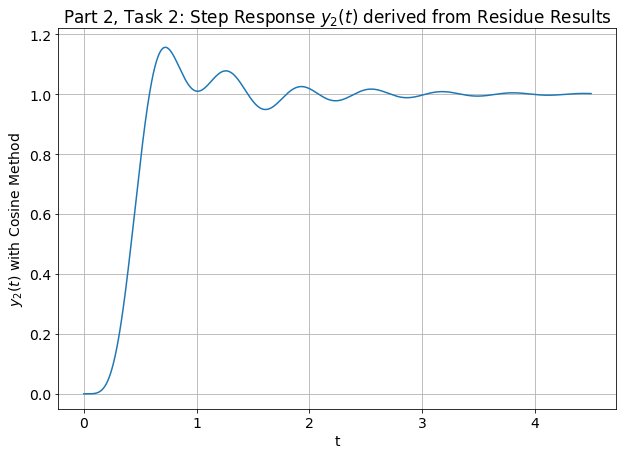
\includegraphics[scale = 0.52]{Part2-Task2.png}\\[1.0 cm]
\end{center}

The second convolution plot is between $f_2(t)$ with $f_3(t)$. If we attempted a graphical convolution by flipping the exponential again, it is clear that the overlap would match the sharp increase and decrease of $f_3$. This is also supported by the scipy.signal.convolve function results. \\

\begin{center}
	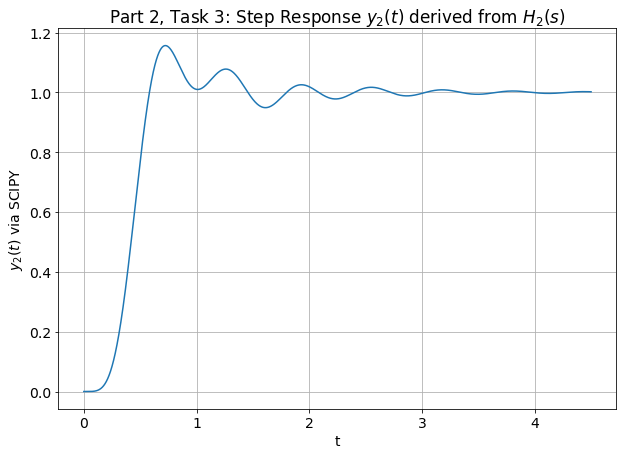
\includegraphics[scale = 0.52]{Part2-Task3.png}\\[1.0 cm]
\end{center}

The final convolution plot for $f_1(t)$ and $f_3(t)$ closely aligns with expectations. The overlap of the graphical convolution increases dramatically and remains a fixed value until the functions pass, causing a chiastic dramatic decrease. The convolution results from the Python package function shown in the bottom subplot match those given by the user-defined function. As all three convolutions agree with those provided by the built-in convolution function, this supports the conclusion that the user-defined convolution function functions properly. \\
	
\begin{center}
	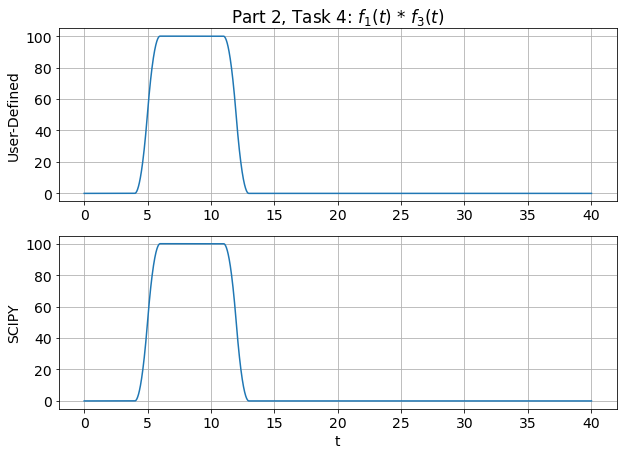
\includegraphics[scale = 0.55]{Part2-Task4.png}\\[1.0 cm]
\end{center}
	
\section{Error Analysis}

The major source of difficulty in this lab was attempting to create the user-defined convolution function. While there were some elements that I proposed correctly would be in the solution such as the nested loops, I struggled with identifying the values to iterate through in order to properly measure the overlap of the two functions. I also failed to correct the error from mismatched function dimensions. The solutions to these issues were not found independently; rather, the code provided by the TA during the lab session and included in this report fixed these problems. 

I also failed to increase the time interval for the convolution result at first. The proper interval was found through initial trial and error and contemplation. After printing the differing dimensions several times, the necessary time interval was found.
		
\section{Questions}
	
1. I worked alone when attempting to find the solution in this lab. The process involved rereading the section in Dr. Sullivan's textbook on convolution, sketching examples, and implementing small sections of test code. Ultimately, the solution was only found through demonstration by the lab TA. \\
	
2. As mentioned in the error analysis, the most difficult part of this lab for me was determining how the two functions could be iterated through to find the overlap. In my attempt to solve this problem individually, I tried to create two variables for t and $\tau$ to index two nested loops. I never assigned the right value to these two. I tried to directly input the values I deemed necessary, but was met with dimension errors. The problem-solving process was halted by the in-class demo. \\
	
3. I first approached writing the code with an analytical convolution in mind. I tried to directly input a summation that would capture the idea of the convolution. I attempted this approach because it seemed direct and I thought I could find a correlation between variables in the code and in the equation. When I hit a wall, I switched to considering a graphical convolution and began sketching the process. This was done to try to look at the big picture and understand how the convolution operated and what it actually accomplished. \\
	
4. The lab tasks, expectations, and deliverables are all clearly communicated. \\
	
\section{Conclusion}
	
This lab facilitated a deeper understanding of the convolution and its properties.  In creating a user-defined convolution function, we learned how to append to a numpy array and the importance of keeping track of array dimensions. We also expanded our ability to think critically about how to implement an operation, improving our problem-solving skills. As the results of this lab aligned with expectations across the board, we could call the lab successful. It does not feel like such a success, however, since the solution was handed out instead of earned with a satisfying breakthrough. Despite this, I do feel that I gained further understanding of the convolution as well as new insight into how to analyze a problem. The development of these skills will surely be useful for labs going forward.

\newpage
\begin{thebibliography}{111}
		
	\bibitem{S}
Sullivan, Dennis M. (2018) {\it  Signals and Systems for Electrical Engineers I}. Nevada: CreateSpace Independent Publishing Platform.
		
		
\end{thebibliography}
\end{document}

% Lab Report based on template created by Roza Aceska.